
%Copyright (C) 2016 by Krishneel@JSK Lab, The University of Tokyo

\documentclass{standalone}
\usepackage{footnote}
\usepackage{hyperref}
\usepackage{graphicx}

\begin{document}

\subsection{Software}

The software, including motion planning, visual perception and virtual simulation, are developed on the ROS robot operating system, and we use Gazebo for performing simulations \footnote{\url{https://github.com/start-jsk/jsk_mbzirc}}. We use the Gazebo simulator for testing and planning our strategy and for customizing our hardware and software. The visual perception component carries out target (heliport) localization of the moving vehicle, and we plan the efficient approaching and landing strategy based on the motion of both the UAV and the vehicle. Since we use Nvidia TX1 embedded processor for fast computations on GPU, our algorithms for \textit{task 1} and \textit{task 3} are developed in CUDA-C, C/C++ and Python. 

% \begin{figure}[t]
%   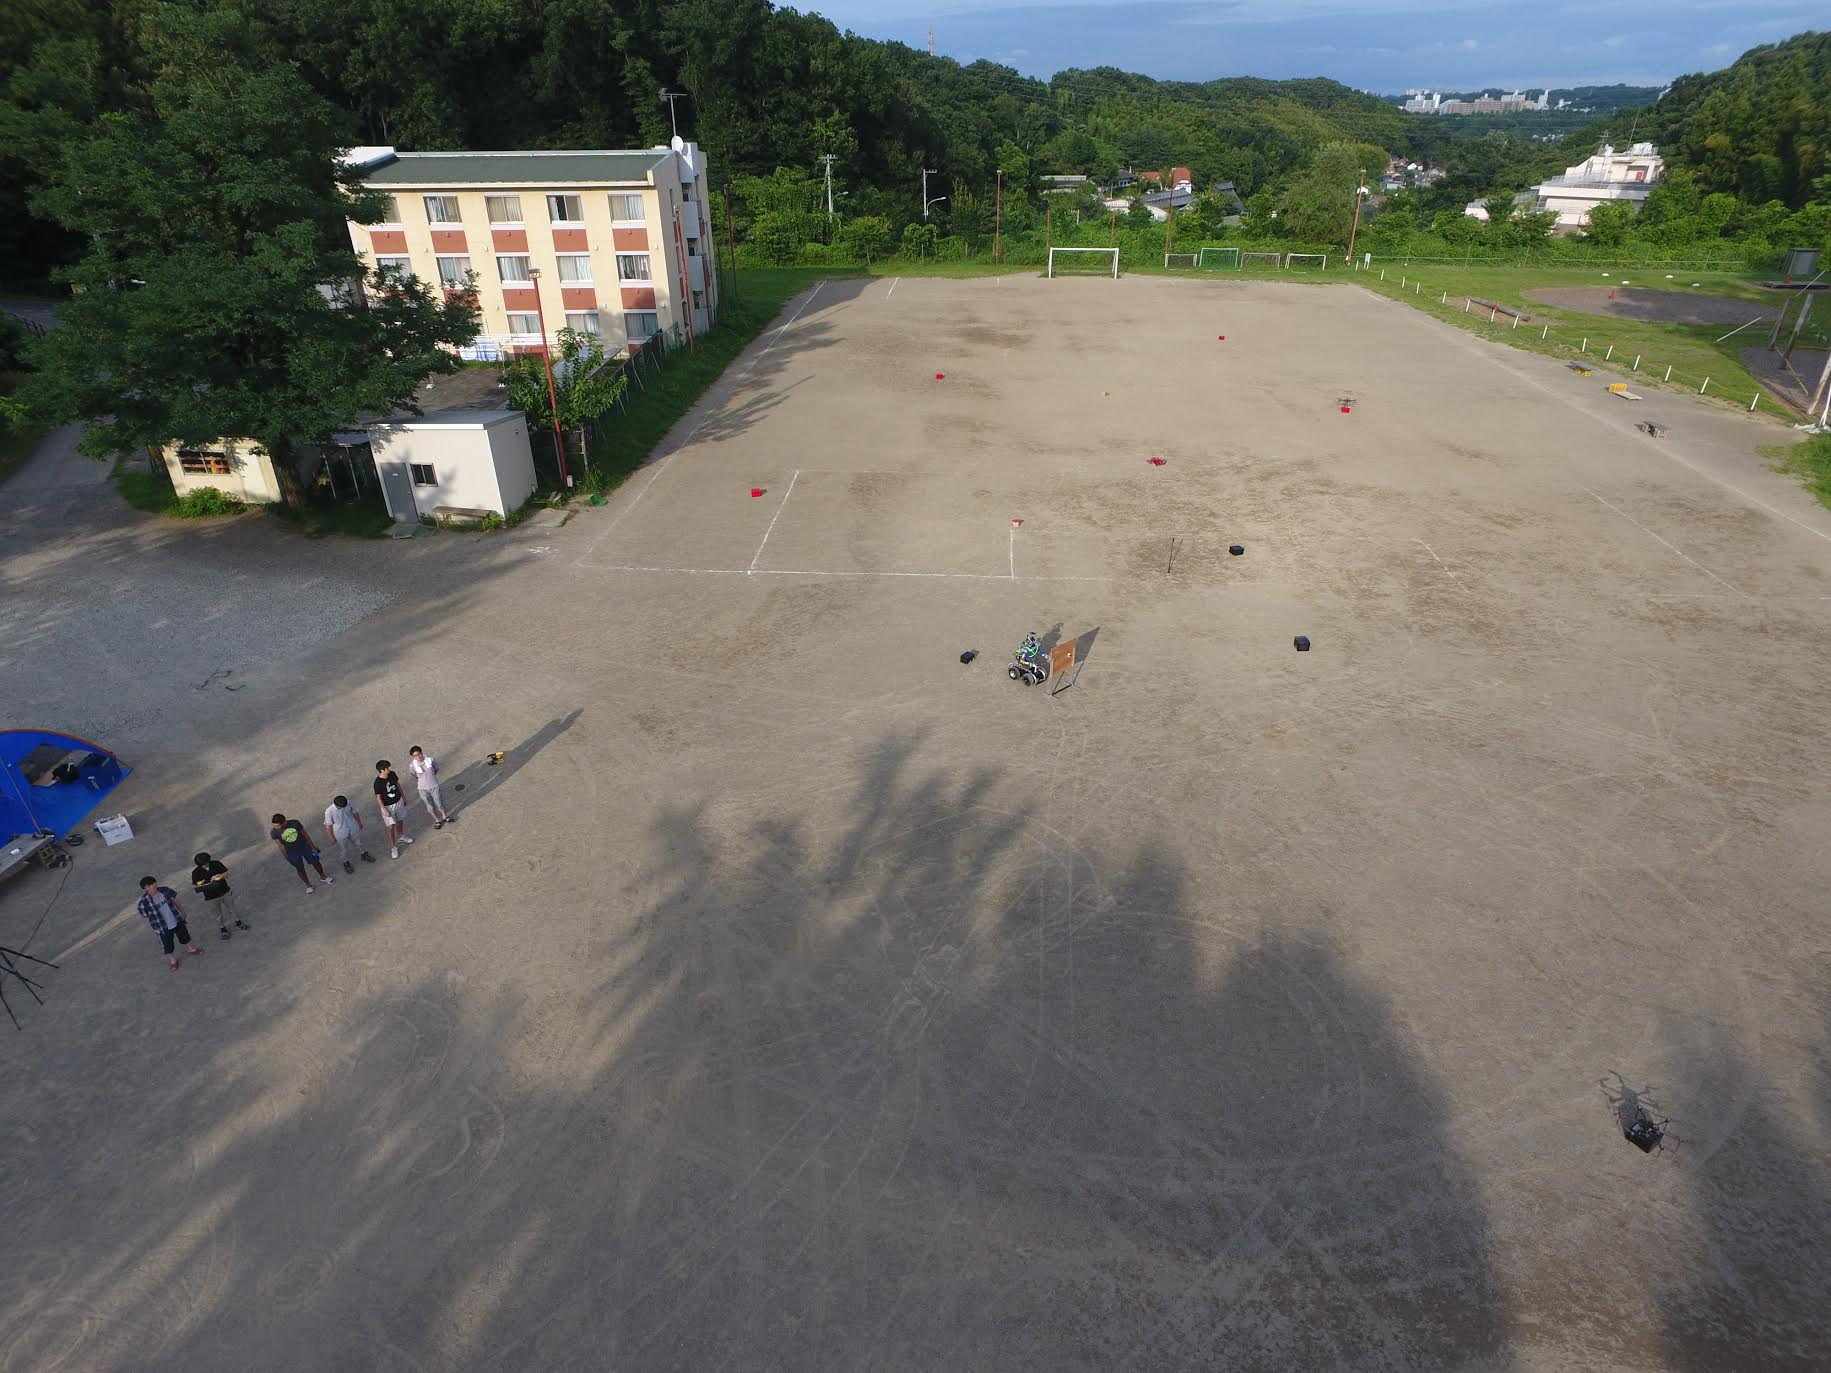
\includegraphics[width=\columnwidth, trim={2cm 5cm 3cm 7cm},clip]{sections/task1/images/testbed}
%   \caption{Testbed for outdoor testing in Hachioji, Tokyo, Japan}
% \end{figure}


\subsection{General Approach}

%\textbf{Vehicle And Heliport Detection}: 
We use the heliport model to train a linear classifier for detection of the landing region. Since heliport model is known, it is used as an a priori for learning. Once the heliport is detected, a visual object tracker running in real time on-board is autonomously initialized to start tracking the target region. We use a robust tracking algorithm with efficient drift compensation algorithm to avoid lost of target when the UAV is in motion. Our visual tracking algorithm is also able to recover the target even if it went completely out of view. Once the target is localized, the UAV uses pose information from the visual tracker to navigate towards the target. 

\subsection{Future Plans}
The future work on hardware platform for task 1 includes the design of landing gear which enables to attach to a moving heliport. The sturdy and light protector of UAV is another issue to avoid the crash while hitting to the truck.
The future work on software for task 1 involves testing the completed software on the customized UAV which is currently under development. This involves fine tuning the current simulator version of our software. Considering the challenges in outdoor environment such as abrupt changes in image space, winds speeds etc. the landing strategy might vary significantly from the simulator version. One very important aspect of autonomous systems which we like to implement is the ability of the UAV to recover from erroneous decision, false positives that might result in highly cluttered and unstructured scene. To achieve this we plan to generate a map of the environment at the beginning for efficiently localizing the vehicle and for trajactory mapping. The idea is that, the UAV can use the constructed map, to eliminate regions that produces false positives. However, the current limitation is the time required for generating the map which we aim to reduce using the idea of task oriented solution.

\end{document}
